% Tabela: Equivalencias ECC
\begin{table}[H]
	\centering
	\caption{Equivalência de chaves entre diferentes algoritmos criptográficos.}
	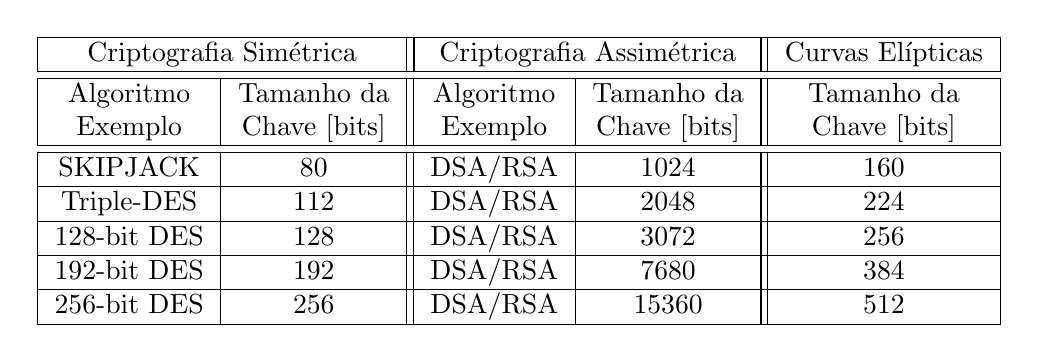
\begin{tikzpicture}
		
		\node[thick, align=center] (table) {
			\begin{tabular}{ |c|c||c|c||c| }
				\hline
				\multicolumn{2}{ |c|| }{Criptografia Simétrica} &
				\multicolumn{2}{ |c|| }{Criptografia Assimétrica} &
				Curvas Elípticas
				\\ \hline \hline
				
				Algoritmo & Tamanho da   & Algoritmo & Tamanho da   & Tamanho da \\
				Exemplo   & Chave [bits] & Exemplo   & Chave [bits] & Chave [bits]
				\\ \hline \hline
				
				SKIPJACK    & 80  & DSA/RSA & 1024  & 160 \\ \hline
				Triple-DES  & 112 & DSA/RSA & 2048  & 224 \\ \hline
				128-bit DES & 128 & DSA/RSA & 3072  & 256 \\ \hline
				192-bit DES & 192 & DSA/RSA & 7680  & 384 \\ \hline
				256-bit DES & 256 & DSA/RSA & 15360 & 512 \\ \hline
			\end{tabular}
		};

	\end{tikzpicture}
	\label{tab:equivalencias_ecc}
\end{table}